\documentclass{oblivoir}
\usepackage{graphicx} % Required for inserting images
\usepackage{verbatim}
\usepackage{float}
\usepackage[a4paper, total={6in, 9in}]{geometry}
\setcounter{tocdepth}{5}
\setcounter{secnumdepth}{5}
\hypersetup{
    colorlinks=true,
    linkcolor=blue
}

\title{HW5}
\author{C311054 박민서}
\date{2025년 6월 19일}

\begin{document}

\maketitle

\section{Insertion Sort}
\subsection{Prolog 문법}
\paragraph*{append}
첫번째 리스트와 두번째 리스트를 이은 리스트가 세번째 리스트일 때 참이 된다.
\begin{verbatim}
?- append([a,b], [c], X).
X = [a,b,c].
\end{verbatim}

\paragraph*{부등호}
 부등호는 다음과 같이 쓴다.
 \begin{verbatim}
 ?- 2>=3.
 false.
 ?- 2=<2.
 true
 \end{verbatim}

\subsection{작동방식}

sorting을 호출하면 빈 리스트를 두번째 인자로 추가해 insert\_sort가 호출된다.
insert\_sort는 첫번째 리스트의 첫번째 원소를 두번째 리스트에 삽입하는 insert를 호출한다. insert는 삽입할 리스트가 빈 리스트이면 그대로 원소를 넣은 리스트를 세번째 인자로 갖는다. 삽입이 완료된 리스트와 첫번째 원소가 제거된 리스트를 합치면 각 단계에서의 리스트 상태가 된다. 따라서 합친 리스트를 출력하고 줄바꿈을 한다. insert\_sort는 tail부분과 삽입이 완료된 리스트를 인자로 하여 재귀호출한다. insert는 삽입될 원소와 삽입할 리스트의 첫번째 원소를 크기비교하여 삽입할 원소가 더 크다면 리스트의 tail부분을 삽입할 리스트로 하여 재귀호출하고, 작거나같다면 그 원소를 리스트의 head로 하여 삽입한다.

\begin{figure}[H]
    
    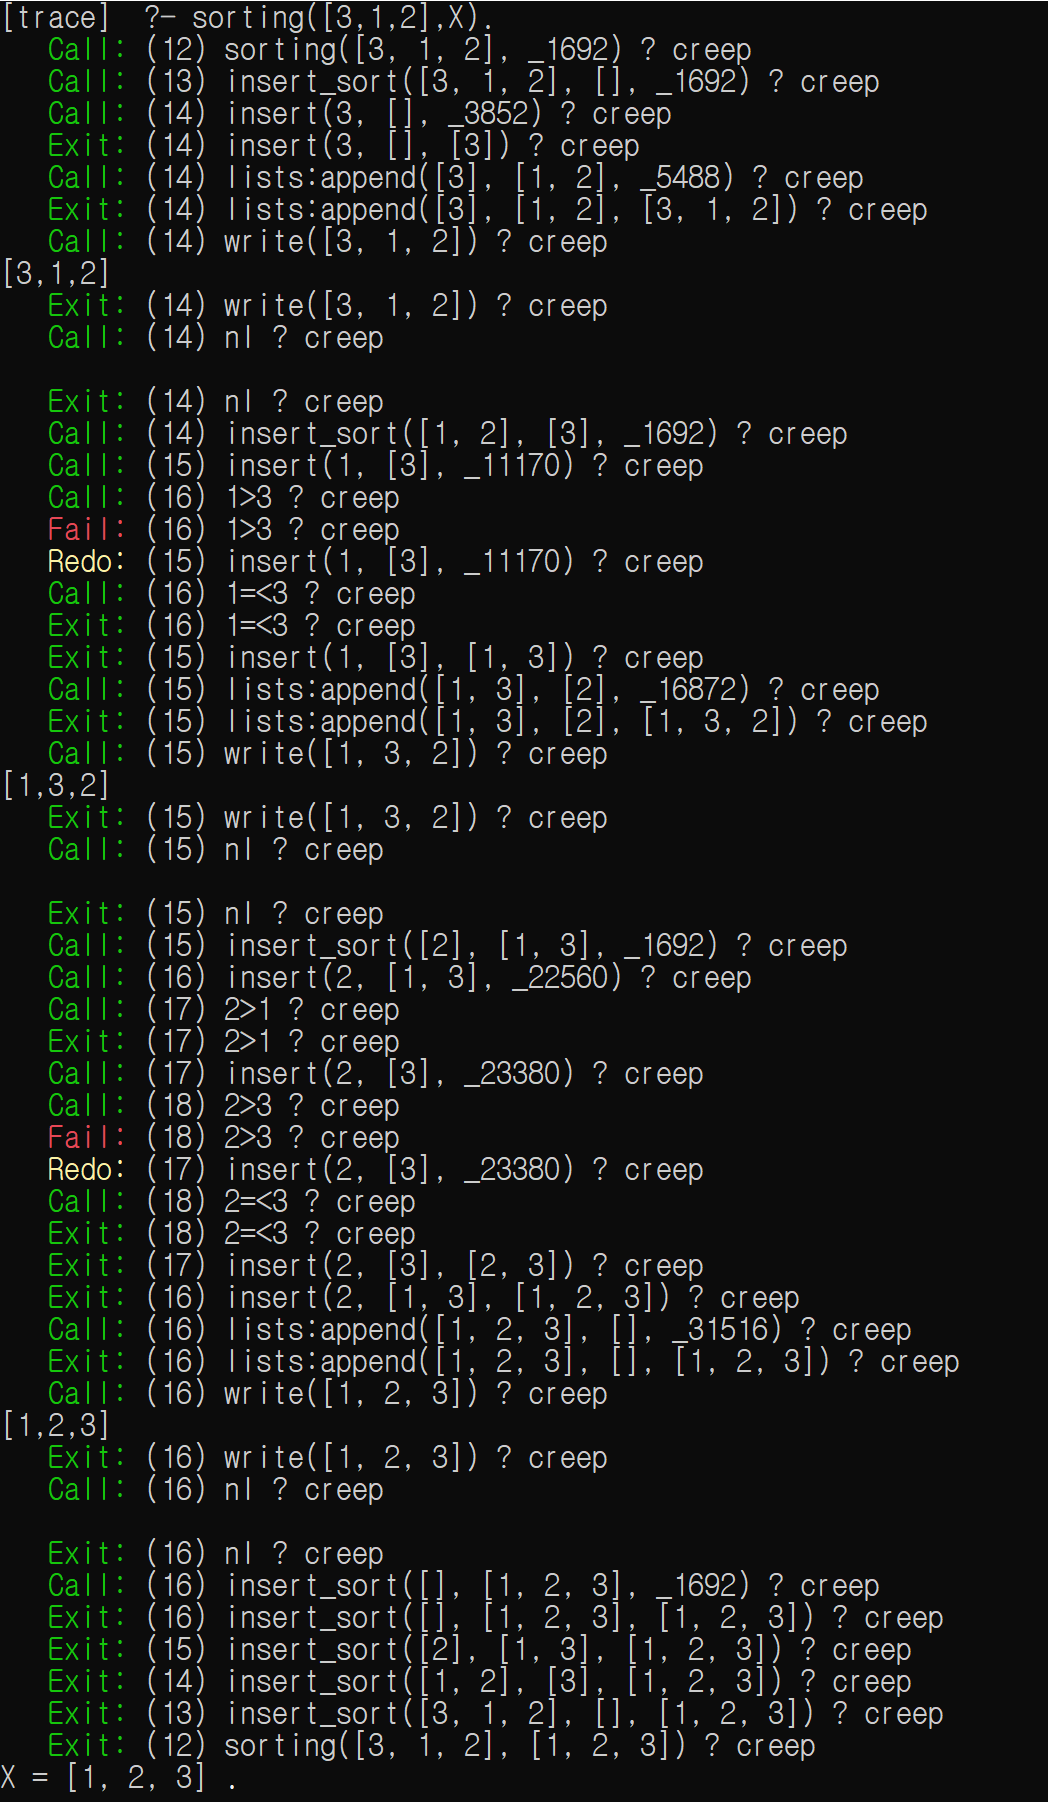
\includegraphics[width=0.5\linewidth]{trace_a.PNG}
    
\end{figure}


\subsection{코드}
\begin{verbatim}
sorting(Init,Sorted):-insert_sort(Init,[],Sorted).  %1

insert_sort([H|T],Temp,Sorted):-    %2
        insert(H,Temp,Inserted),    %3
        append(Inserted,T,C),write(C),nl,   %4
        insert_sort(T,Inserted,Sorted). %5
insert_sort([],Li,Li).  %6

insert(X,[Y|T],[Y|Inserted]):-X>Y,insert(X,T,Inserted). %7
insert(X,[Y|T],[X,Y|T]):-X=<Y.  %8
insert(X,[],[X]).   %9
\end{verbatim}
주석의 번호별로 설명하겠다.
\paragraph*{1}
Init에는 정렬하고자하는 리스트를 넣는다. Sorted에는 정렬된 리스트가 들어간다.

\paragraph*{2}
첫번째 인자는 정렬되지 않은 리스트의 뒷부분으로 head와 tail로 나눠지고 Temp는 삽입정렬된 리스트의 앞부분이다. Sorted에는 모든 정렬이 완료된 리스트가 들어간다.

\paragraph*{3}
리스트의 정렬되지 않은 부분의 첫번째 원소인 H를 정렬된 리스트인 Temp로 삽입하고 그 결과가 Inserted에 들어간다.

\paragraph*{4}
Inserted는 이제 H까지 삽입정렬된 상태이고 H를 제외한 부분인 T가 아직 정렬되지 않은 뒷부분이다. 따라서 이 둘을 합친 C가 현재 리스트의 상태이므로 출력하고 줄바꿈한다.

\paragraph*{5}
이제 T와 Inserted를 인자로 하여 insert\_sort를 재귀호출한다. Sorted에는 전체 정렬이 완료된 리스트가 들어가므로 그대로 전달한다.

\paragraph*{6}
insert\_sort 재귀의 종료조건은 첫번째 인자가 빈 리스트가 됐을 때이다. 즉 모든 원소를 두번째 리스트에 삽입하였다는 뜻이므로 두번째 리스트가 그대로 세번째 인자(정렬이 완료된 리스트)가 된다.

\paragraph*{7}
삽입될 원소가 삽입할 리스트의 첫번째 원소보다 크다면 뒷부분에 삽입해야되므로 삽입할 리스트를 tail로 하여 재귀호출한다. body의 insert에서 X가 삽입된 리스트인 Inserted와 Y를 합친 리스트가 insert의 세번째 인자가 되어 insert\_sort에서 Inserted로 사용된다.

\paragraph*{8}
삽입될 원소가 삽입할 리스트의 첫번째 원소보다 작거나 같다면 리스트의 첫번째 원소로 삽입된다.

\paragraph*{9}
만약 삽입할 리스트가 빈 리스트면 그대로 원소를 삽입한 리스트가 세번째 인자가 된다. 재귀의 종료조건으로도 사용된다.

\subsection{실행결과}
\begin{figure}[h]
   
    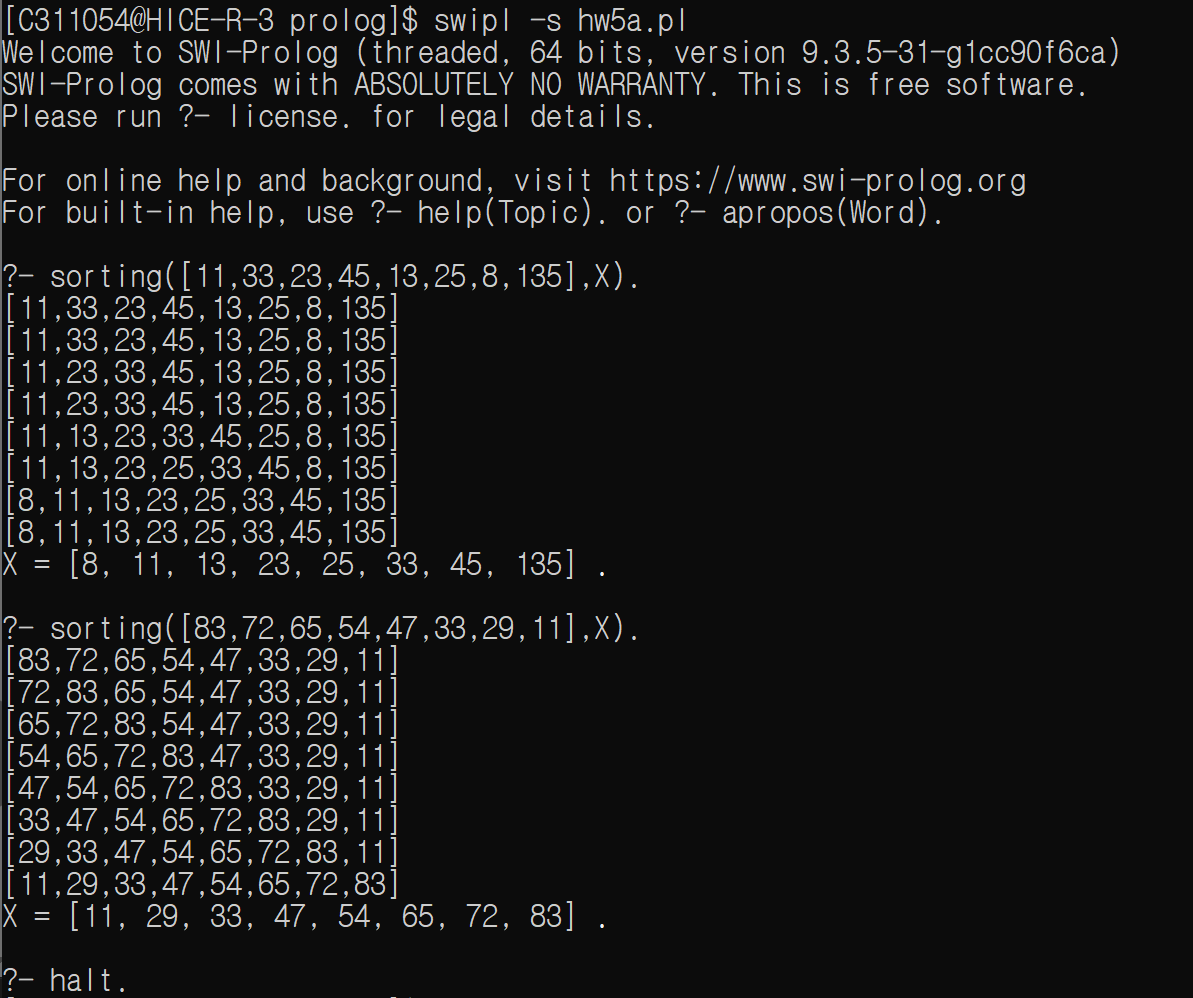
\includegraphics[width=0.5\linewidth]{result_a.PNG}

\end{figure}

\section{N-Queen problem}
\subsection{Prolog 문법}
\paragraph*{규칙은 위에서부터 매칭된다.}
\begin{verbatim}
f(X):-...
f(0):-...
?-f(0). %첫번째 규칙에 매칭 후 fail시 두번째 규칙에 매칭
\end{verbatim}
\paragraph*{빈 리스트는 head와 tail로 나눌 수 없다.}
\begin{verbatim}
f([H|T]):-...
f([]):-...  %빈 리스트는 여기에 매칭
\end{verbatim}
\paragraph*{규칙의 인자로 수식을 쓸 수 없다.}
\begin{verbatim}
f(X):-g(X+1). %수식이 평가되지 않음.
f(X):-X2 is X+1, g(X2). %올바른 방법
\end{verbatim}

\subsection{작동방식}
trace가 긴 관계로 필요한 부분만 잘라 설명하겠다.


\begin{figure}[h]
 
    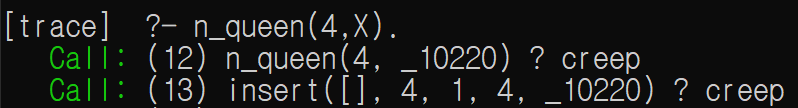
\includegraphics[width=0.5\linewidth]{trace_b1.PNG}
   
\end{figure}
n\_queen은 insert를 호출한다. insert는 특정 행, 열에 퀸을 놓는 역할이다. insert는 퀸을 놓기 전에 그 자리에 퀸을 놓을 수 있는지 검사하는 check을 호출한다.

\begin{figure}[h]
  
    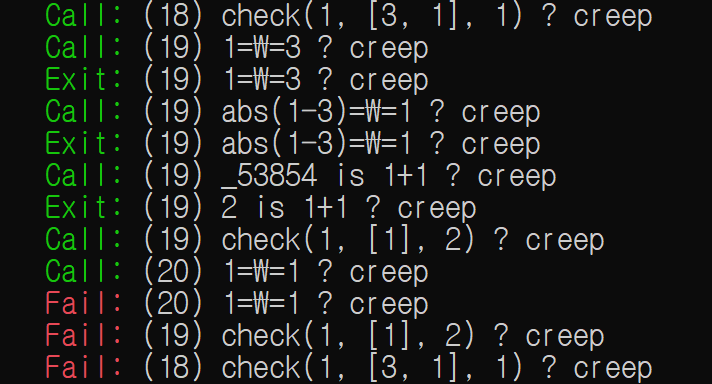
\includegraphics[width=0.5\linewidth]{trace_b2.PNG}
   
\end{figure}
check은 삽입하고자 하는 원소가 기존 리스트의 원소들과 충돌하지 않는지 검사한다. 리스트의 head와 충돌여부를 검사하고 tail을 리스트로 하여 재귀호출한다. 

\begin{figure}[H]
  
    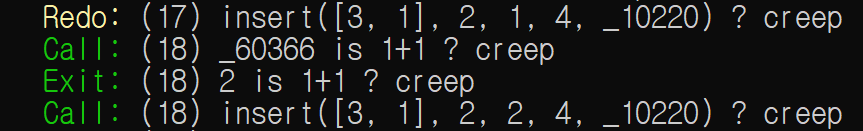
\includegraphics[width=0.5\linewidth]{trace_b3.PNG}
    
\end{figure}
check이 fail됐다면 다음 열로 옮겨 다시 insert를 호출한다.

\begin{figure}[H]

    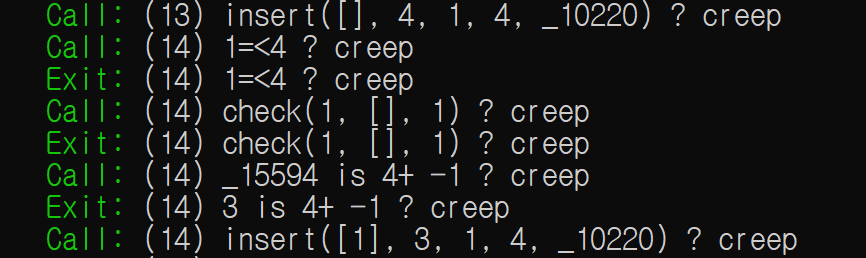
\includegraphics[width=0.5\linewidth]{trace_b4.PNG}
   
\end{figure}
check이 성공했다면 다음 행의 첫 열에서 insert를 호출한다.

\begin{figure}[H]
  
    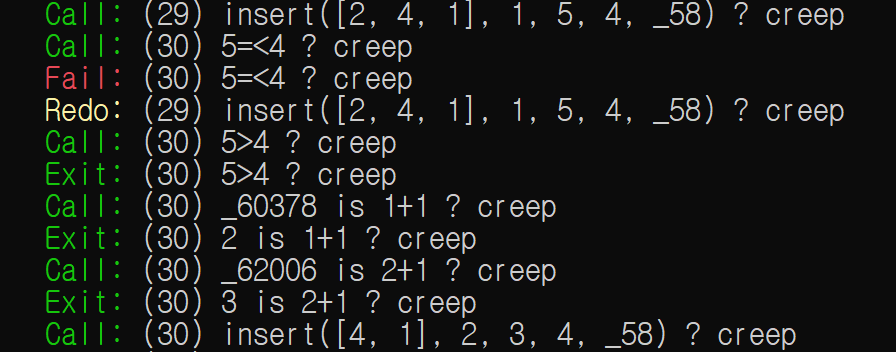
\includegraphics[width=0.5\linewidth]{trace_b5.PNG}
    
\end{figure}
만약 열이 범위를 벗어나면 해당 행에는 배치할 곳이 없다는 뜻이므로 이전 행의 퀸을 다음 열로 이동시켜 다시 insert를 호출한다.

\begin{figure}[H]
  
    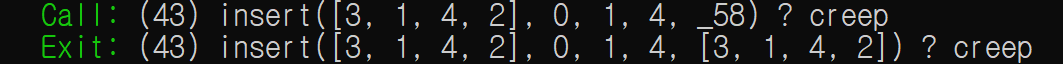
\includegraphics[width=0.5\linewidth]{trace_b6.PNG}
   
\end{figure}
마지막 행까지 모두 채웠다면 리스트를 반환한다.

\subsection{코드}
\begin{verbatim}
n_queen(N,X):-insert([],N,1,N,X).   %1

insert(Li,0,_,_,Li).    %2
insert(Li,Row,Col,N,X):-    %3
        Col=<N, !,  %4
        (check(Col,Li,1)->  %5
        Row2 is Row-1, insert([Col|Li],Row2,1,N,X); %6
        Col2 is Col+1, insert(Li,Row,Col2,N,X)).    %7
insert([H|T],Row,Col,N,X):- %8
        Col>N,  %9
        Row2 is Row+1, H2 is H+1, insert(T,Row2,H2,N,X).  %10

check(Target,[H|T],Dist):-  %11
        !,Target=\=H,   %12
        abs(Target-H)=\=Dist,   %13
        Dist2 is Dist+1, check(Target,T,Dist2). %14
check(_,[],_).  %15
\end{verbatim}

\paragraph*{1}
n\_queen은 빈 리스트의 N행 1열에서 시작하는 insert를 호출한다. insert의 인자는 3번에서 자세히 설명한다. prolog의 특성 상 리스트의 앞부분에 원소를 추가하는 것이 편리하기때문에 마지막 행에서 시작하도록 했고 예시 출력과 맞추기 위해서 마지막 행의 열번호가 작은 순으로 시작하도록 했다.

\paragraph*{2}
0행에 대한 insert가 호출되었다는 것은 1부터 N행 까지 모두 퀸을 배치했다는 것이므로 X에 그대로 리스트를 넣어준다.

\paragraph*{3}
insert의 인자는 퀸을 배치하는 리스트, 행번호, 열번호, 입력값으로 받은 퀸의 갯수(체스판의 변의 길이), 결과를 넣을 리스트 X로 이루어져있다. 리스트의 i번째 원소인 j는 체스판의 i행 j열에 퀸을 배치했음을 나타낸다.

\paragraph*{4}
이 규칙은 열번호가 범위내일 경우이다. 범위 밖의 경우는 insert의 첫번째와 세번째 규칙에서 처리한다. 문법에서 설명한 매칭 순서에 따라 행번호가 0이 되는 경우(2번줄)는 이 규칙이 적용되지 않도록 더 위에 배치해야한다. 그리고 기본적으로는 범위내일 것이기 때문에 이 규칙을 세번째 규칙보다 위에 써서 fail,redo의 횟수를 줄였다. 또한 범위 검사를 통과한 뒤에는 cut을 사용해 세번째 규칙으로 redo를 하지 않도록 하였다.

\paragraph*{5}
해당 열에 퀸을 배치할 수 있는지 검사하기 위해 check을 호출한다. 인자로 열번호와 현재까지 퀸을 배치한 리스트, 1을 초기값으로 전달한다. check의 인자에 대해서는 11에서 설명한다.

\paragraph*{6}
만약 check가 성공했다면 리스트에 퀸을 배치하고 행번호는 1감소, 열은 다시 1에서 시작하여 insert를 호출한다.

\paragraph*{7}
check이 실패했다면 나머지 인자는 그대로, 열번호만 1증가시켜 insert를 호출한다.

\paragraph*{8}
이 세번째 규칙에서는 head와 tail을 사용하기때문에 빈 리스트는 매칭되지 않는다. 따라서 빈 리스트와 N보다 큰 열번호가 인자로 호출되었을 경우는 이 규칙이 아니라 두번째 규칙에 매칭되고 4번줄의 부등식에 의해 fail된다. 이 경우는 모든 퀸을 배치하는 방법이 없다는 뜻이다. N이 2나 3일 때 해당된다.

\paragraph*{9}
열번호가 N보다 크다는 것은 현재 상태에서 해당 행에 퀸을 배치할 수 있는 열이 없다는 뜻이다. 

\paragraph*{10}
현재 배치 상태에서는 더이상 퀸을 놓을 수 없다는 것이므로 기존에 배치되어있던 퀸을 하나 제거하고 원래 배치되었던 열에서 한칸 이동해 insert를 호출한다. 이전행에서 다시 시작하기때문에 행번호를 1증가, 기존의 열번호에서 1증가시키고 리스트는 tail부분으로 하여 호출한다. 행번호는 줄어드는 방향으로, 열번호는 증가하는 방향으로 배치하고 있다는 것을 상기하자.

\paragraph*{11}
check은 현재 배치하고자 하는 퀸의 열번호, 이미 배치되어 있는 퀸들의 리스트, 충돌여부를 비교하는 두 원소 사이의 리스트 상 거리를 인자로 받는다.
거리는 행번호의 차이를 의미한다. 삽입하고자 하는 원소는 이미 리스트에 있는 head의 한 칸 앞에 들어올 것이기때문에 Dist의 초기값은 1로 호출한다.

\paragraph*{12}
check은 Target과 리스트의 head를 비교하는 식으로 재귀반복하여 리스트의 모든 원소와 Target을 비교하는데 만약 한 번이라도 fail한다면 그 Target에 대한 모든 check 재귀호출이 fail되야하므로 cut을 사용해 불필요한 redo를 하지 않도록 한다.
퀸 사이 충돌의 첫번째 조건은 열번호가 같은 경우다. Target과 리스트의 head가 같은 숫자면 fail이다. 각 행마다 퀸을 하나씩 배치하기때문에 행번호가 같은 경우는 없다. 

\paragraph*{13}
충돌의 두번째 조건은 같은 대각선 상에 위치하는 경우이다. 이는 열번호의 차와 행번호의 차가 같은 경우인데 리스트에 열번호가 들어있기 때문에 열번호의 차는 abs(Target-H)가 되고 행번호의 차는 Dist라는 인자로 전달된다. Dist는 항상 양수이므로 절댓값을 취하지 않아도 된다. 

\paragraph*{14}
head에 대한 충돌검사를 통과하였다면 tail을 리스트로 넘겨 다음 원소에 대해 검사한다. Dist는 1씩 증가한다.

\paragraph*{15}
빈 리스트가 들어왔다면 모든 원소에 대해 검사가 통과되었다는 뜻이다.

\subsection{실행결과}
\begin{figure}[H]
  
    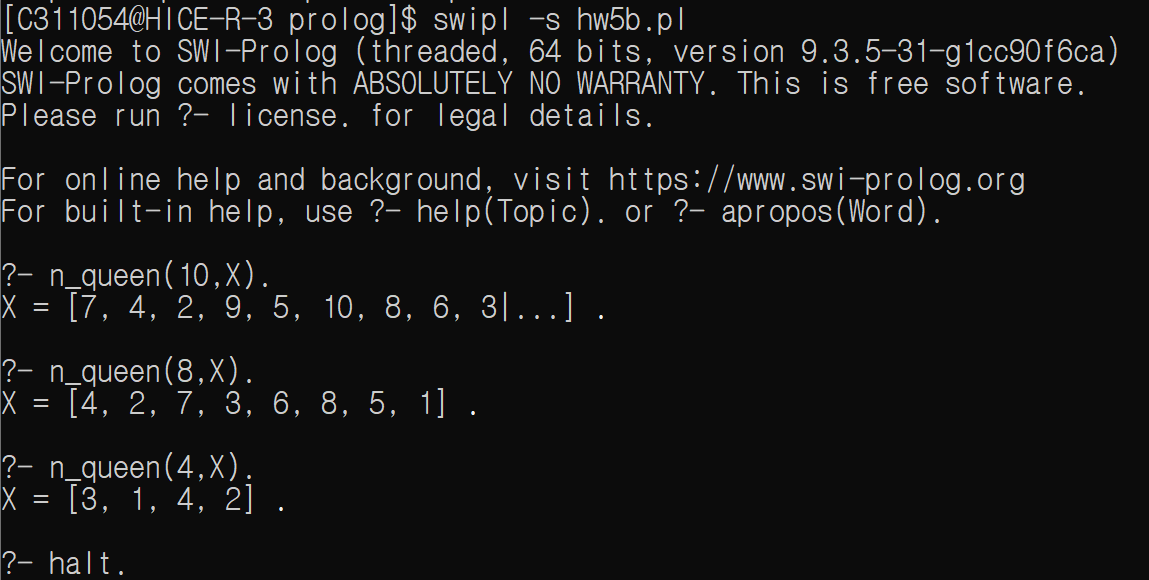
\includegraphics[width=0.5\linewidth]{result_b.PNG}
   
\end{figure}

\section{어려웠던 점}
명령형 언어에만 익숙해져 있어서 논리형 언어의 체계를 이해하는 것부터가 어려웠고 그 체계를 이용해 코드를 작성하는 것도 어려웠다. 명령형 언어가 문제의 해결 과정을 서술한다면 논리형 언어는 문제의 답을 명시하고 거기에 맞는 값을 찾는 식이라고 느꼈다. 하지만 어떤 규칙을 적용할 때 일단 규칙의 head부분에서 변수의 값을 할당해놓고 body의 조건을 하나씩 적용해나가는 것은 다른 언어의 함수와 비슷한 면으로도 보였다. 규칙 적용 중 fail을 한 뒤 redo하는 trace의 흐름과 cut의 쓰임도 처음에는 이해하기 어려웠다.


\end{document}
